\chapter{Avionics and Airframe}\label{cha:avionics-airframe}

This chapter discusses XCSoar as a subsystem of the aircraft.  It
covers the integration of XCSoar with external devices, including GPS,
switches and sensors, and aircraft radio transceivers and other
devices.  Integration with FLARM is covered in
Chapter~\ref{cha:airspace}, and integration with variometers is
covered in Chapter~\ref{cha:atmosph}.

\section{Battery life}

Most modern PDAs are designed for short sporadic use and so do not
have a very good battery capacity when considering the duration of
cross-country soaring flights.  It is recommended that the PDA be powered
externally, via an appropriate voltage converter connected to the glider battery. 
This installation should be performed by appropriately qualified personnel, 
and should contain a fuse and a manual isolation switch.

The greatest cause of power drain by the PDA is the LCD back-light,
however domestic PDAs are not particularly bright so they may need to
have the back-light up full. However, for EFIS systems such as Altair,
it is recommended to use the lowest back-light settings that are
comfortable.

When operating PDAs under internal battery, XCSoar detects a low
battery condition and allows the operating system to shut down and
preserve the memory.  In addition, it can be set up to blank the
screen after a period of inactivity, so that it can reduce the power
consumption.  When the screen is blanked, pressing one of the hardware
buttons on the PDA activates the screen again.  When a status message
is issued by the system, the screen becomes activated.

Another way to help conserve battery power is to reduce the
computational load by turning off certain features.  Drawing terrain
and long snail trails contribute significantly to the CPU load.

For Altair/Vega systems, the external supply voltage is displayed on
the system status dialogue (see Section~\ref{sec:system-status}).

For other embedded platforms, a \infobox{Battery} InfoBox is available that 
displays the available battery life remaining, as well as the charge state 
(AC on--charging, or AC Off--operating off internal battery power).

\section{GPS connection}

XCSoar requires a 3D GPS fix for its navigation functions.

\subsection*{GPS status}

GPS status icons and text may appear on the bottom edge of the
map display to indicate:

\begin{tabular}{c c}%{c c}
\includegraphics[angle=0,width=0.75cm,keepaspectratio='true']{icons/gps_acquiring.pdf} & \includegraphics[angle=0,width=0.75cm,keepaspectratio='true']{icons/gps_disconnected.pdf}\\
(a) & (b)
\end{tabular}

\begin{description}
\item[Waiting for GPS fix (a)]  Better reception
  or additional time to search for satellites is required. The GPS may have a 2D fix.
  The aircraft symbol disappears while there is no 3D fix.
\item[GPS not connected (b)]  No communication with the GPS is received.
  This indicates an error in the comm port settings or the GPS device may
  be disconnected or switched off.
\end{description}

When the GPS is not connected for more than one minute, XCSoar automatically 
attempts to restart communication with the device and will then resume waiting. 
This method has shown to provide the most reliable way of recovering from 
communication errors.

XCSoar can handle up to two GPS sources and it uses them to provide redundancy. 
The sources are configured on the System Configuration screen, on the page 
entitled "Devices".  Device A is the primary GPS data source and Device B is 
the secondary source.

During operation, if the primary GPS source drops out, XCSoar will use the GPS 
data from the secondary source.  If both sources have valid fixes, the secondary 
source is ignored.  For this reason, it is recommended to have the GPS source 
with the best antenna or most reliable operation as the primary source (i.e. Device A).

\subsection*{GPS altitude}

Some older GPS units (and some new ones) do not output altitude
relative to mean sea level, rather they output elevation with respect
to the WGS84 ellipsoid.  XCSoar detects when this occurs and applies
the ellipsoid to geoid offset according to an internal tabulated data
at two degree spacing.  This is not required for FLARM units or Altair
Pro, which correctly output MSL altitude.

\section{Switch inputs}

XCSoar supports monitoring of switches and sensors connected to the
host computer, for the purpose of providing situational awareness
feedback, alerts, or as general-purpose user-interface input devices.
Several mechanisms are available for interfacing to switches and
sensors:
\begin{description}
\item[Serial device]  Certain intelligent variometers such as
 triadis engineering's Vega have multiple airframe switches
 and pass this information on to the PDA or EFIS as special
 NMEA sentences.
\item[1-Wire device]  triadis engineering's Altair glide computer
 and Vega variometer provide a 1-Wire peripheral bus to which
 various digital and analog sensors can be attached.
\item[Bluetooth device]  Many Pocket PC devices support wireless
 connection to a Bluetooth Game-Pad device that has several buttons.
 This is more suited to user-interface input devices than airframe
 monitoring.
\end{description}

A custom `input events' file determines how switch and sensor
inputs are processed.

A standard set of airframe inputs are defined as:
\begin{itemize}
\item Airbrake
\item Flap position (positive/landing flap, neutral, negative/reflex)
\item Landing gear
\end{itemize}

This set is expected to expand to include engine and fuel monitoring.

Other logical inputs from Vega include computed quantities relating to
specific airframe alerts and aircraft operating envelope warnings, for
example ``airbrake extended and gear retracted''.  

Refer to the Vega documentation %and {\em XCSoar Advanced Configuration Manual}
for more details on switch inputs and how they may be used.

\section{Vega switch dialogue}

A dialogue displaying switch states for the Vega variometer
is available from the menu.
\menulabel{\bmenu{Config 3}\blink\bmenu{Vega}\\
\bmenut{Airframe}{Switches}}

This dialogue is updated in real-time, allowing the pilot
to check the correct functioning of switches during daily
inspection tests or before takeoff. 

\begin{center}
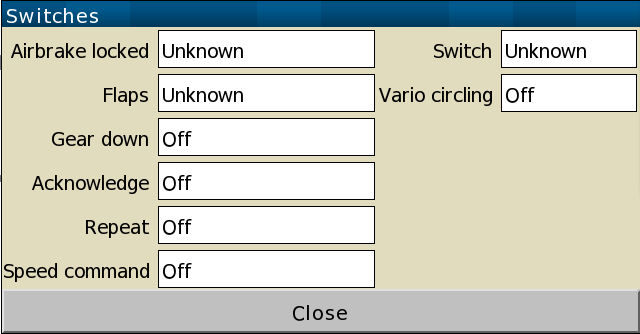
\includegraphics[angle=0,width=0.7\linewidth,keepaspectratio='true']{figures/dialog-switches.png}
\end{center}

\section{Slave mode}

A device type in the configuration settings, ``NMEA Out'' is defined
for use in joining two Altair or PDA systems in a master-slave mode.
In the master, the second com device can be set to NMEA Out, and all
data received in the first com device (as well as outgoing data) will
be sent to the slave.  

As an example where two Altairs are being connected together, in the
slave, the first com device can then be set to ``Vega'' or ``Altair
Pro'' and this system receives all data as if it came from the
Master's GPS and connected instruments (Vega, FLARM etc).


\section{System status}\label{sec:system-status}

The system status dialogue is
\menulabel{\bmenu{Info 2}\blink\bmenu{Status}}
used primarily as a systems check, to see how the glide computer and the 
connected devices are performing.  This is accessed via the menu 
and then selecting the tabular {\bf System}.
\sketch{figures/status-system.png}

All dynamic values (e.g.\ battery voltage, number of satellites in
view) are updated continuously.

\section{Multiple devices}

You can configure up to two external devices, connected at the same
time (few PDAs have two serial ports, but Bluetooth can handle any
number of concurrent connections).

When both provide a valid GPS fix, the first one is chosen by XCSoar,
and the second GPS fix is ignored.  As soon as the first device fails,
XCSoar switches to the second one automatically, until the first one
recovers.

The same is true for all values (barometric altitude, vario, airspeed,
traffic, ...): XCSoar prefers the first device, and uses the second
device only for values that are not received from the first one.

Example: first device is a CAI 302, and the second device is a FLARM.
That gives you the best of both: XCSoar has airspeed, vario and
traffic data.


\section{Managing external devices}

The device management dialogue can be accessed from the configuration
menu (third page).  It shows a list of configured external devices,
and it lists what information they provide.

The button ``Reconnect'' attempts to reconnect to the selected
device.  XCSoar reconnects to a failed device periodically, but
sometimes, it might be desirable to trigger that manually.

The button ``Flight download'' is only available with supported IGC
loggers (see \ref{sec:supported-varios} for a list).  Upon clicking,
XCSoar retrieves a list of flights, and asks you to select one.  The
IGC file will be downloaded to the ``\texttt{logs}'' directory inside
\texttt{XCSoarData}.

The button ``Manage'' is enabled when a Vega or a CAI 302 is
connected.  It provides access to special features of these devices,
such as clearing the CAI 302 flight memory, which is needed sometimes
to work around a Cambridge firmware bug.
